\documentclass[tikz]{standalone}
\usepackage{tikz}
\usepackage{amssymb}
\usetikzlibrary{positioning}
\usetikzlibrary{calc}
\usetikzlibrary{arrows,shapes,snakes,automata,petri}
\begin{document}
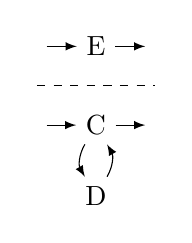
\begin{tikzpicture}
\node[](startC) at (0.25,-1){};
\node[](startE) at (0.25,0){};
\node[](C) at (1,-1){C};
\node[](D) at (1,-1.9){D};
\node[](E) at (1,0){E};
\node[](endC) at (1.75,-1){};
\node[](endE) at (1.75,0){};

\draw[dashed](0.25,-0.5)--(1.75,-0.5);

\path
(startC) edge[-latex]node{} (C)
(startE) edge[-latex]node{} (E)
(C) edge[-latex, bend right]node{} (D)
(D) edge[-latex, bend right]node{} (C)
(C) edge[-latex]node{} (endC)
(E) edge[-latex]node{} (endE);
\end{tikzpicture}
\end{document}